\documentclass[border=3pt]{standalone}
% Preâmbulo compartilhado pelos diagramas TikZ da aula 8 de IHR (Métodos de Pesquisa)
\usepackage[T1]{fontenc}
\usepackage[utf8]{inputenc}
\usepackage{lmodern}
\usepackage{amsmath}
\usepackage{xcolor}
\usepackage{tikz}
\usetikzlibrary{arrows.meta,angles,quotes,decorations.pathmorphing,decorations.pathreplacing,calc,
                positioning,shapes.geometric,shapes.misc,backgrounds,fit,
                math}

% Paleta (mesma dos SVGs originais)
% Paleta da disciplina de IHR: acento azul (#1A6FB5), cor de destaque do tema.
% (o nome "dblue" é mantido para não alterar todos os diagramas)
\definecolor{dblue}{HTML}{1A6FB5}
\definecolor{dorange}{HTML}{B3541E}
\definecolor{dgreen}{HTML}{4A7C59}
\definecolor{dred}{HTML}{9C4B4B}
\definecolor{dcream}{HTML}{F4F1EA}
\definecolor{dshade}{HTML}{DDD7C9}

% Função gaussiana (não normalizada por padrão de escala visual)
\pgfmathdeclarefunction{gauss}{3}{%
  \pgfmathparse{1/(#3*sqrt(2*pi))*exp(-((#1-#2)^2)/(2*#3^2))}%
}

% Estilos comuns (prefixo d... para não colidir com chaves internas do pgf)
\tikzset{
  >={Stealth[length=2mm]},
  dguide/.style={gray!55, dashed, line width=0.4pt},
  daxis/.style={gray!60, line width=0.7pt, ->},
  dbody/.style={fill=black!3, draw=black!80, line width=1pt},
  dacc/.style={draw=dblue, line width=1pt},
  dlbl/.style={black!55, font=\small},
  dsub/.style={black!45, font=\footnotesize},
  dstate/.style={circle, draw=black!80, fill=dcream, line width=1pt,
                 minimum size=17mm, font=\large, inner sep=1pt},
  dobs/.style={circle, draw=black!80, fill=dshade, line width=1pt,
               minimum size=14mm, font=\large, inner sep=1pt},
  dbox/.style={rounded corners=2pt, draw=black!80, fill=dcream, line width=1pt,
               align=center, inner sep=6pt},
  dop/.style={circle, draw=black!80, fill=white, line width=1pt,
              minimum size=6mm, inner sep=0pt, font=\small},
  dtrans/.style={->, dblue, line width=1pt},
  dmeas/.style={->, dorange, line width=1pt},
  dcurve/.style={line width=1pt, dblue},
  dcurveb/.style={line width=1.4pt, dorange},
}

\begin{document}
\hyphenpenalty=10000 \exhyphenpenalty=10000 \tolerance=9999 \emergencystretch=3em
\newcommand{\pc}[3]{% x, y, rótulo
  \draw[dblue, fill=dblue!10, line width=1.5pt, rounded corners=3pt] (#1-0.9,#2-0.6) rectangle (#1+0.9,#2+0.6);
  \draw[dblue, line width=1.5pt] (#1-0.4,#2-0.6) -- (#1-0.5,#2-1.0) -- (#1+0.5,#2-1.0) -- (#1+0.4,#2-0.6);
  \node[font=\large] at (#1,#2-1.45) {#3};}
\newcommand{\pessoa}[2]{% x, y
  \draw[dgreen, fill=dgreen!12, line width=1.5pt] (#1,#2+0.55) circle (0.38);
  \draw[dgreen, fill=dgreen!12, line width=1.5pt, rounded corners=5pt] (#1-0.7,#2-0.95) rectangle (#1+0.7,#2+0.05);}
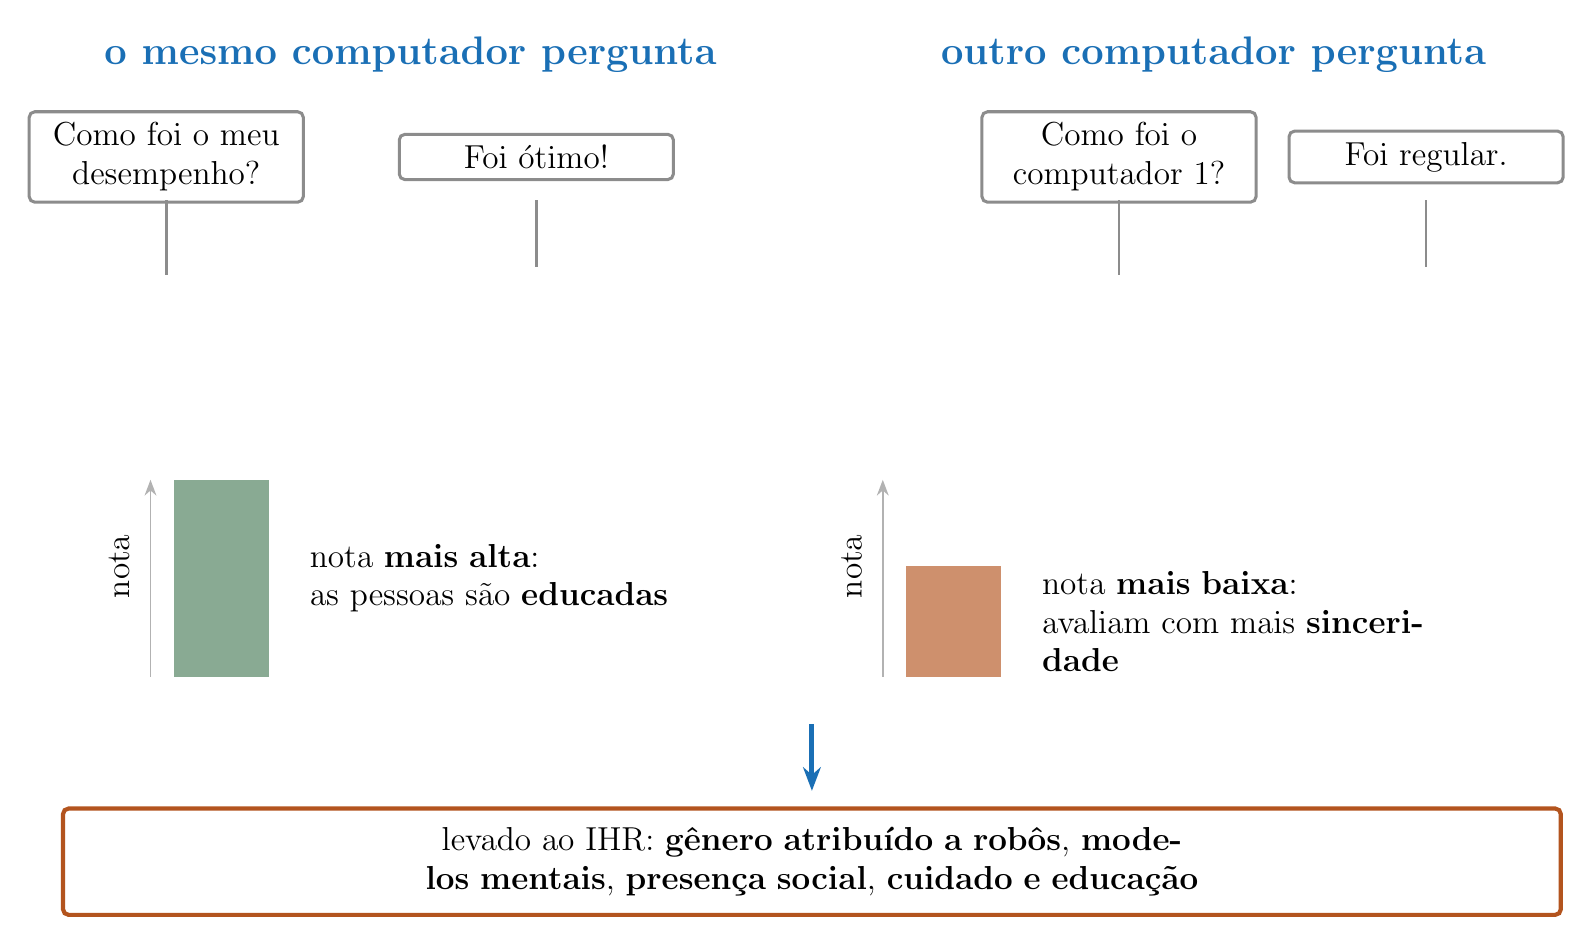
\begin{tikzpicture}[x=1cm,y=1cm]
  \tikzset{bolha/.style={dbox, draw=black!45, fill=white, line width=1.1pt, font=\large, align=center, text width=3.2cm, inner sep=4pt}}
  % ---------- cena A: o mesmo computador pergunta ----------
  \node[font=\Large\bfseries, dblue] at (4.4,9.8) {o \textbf{mesmo} computador pergunta};
  \pc{1.3}{6.3}{computador 1}
  \pessoa{6.0}{6.0}
  \node[bolha] at (1.3,8.5) {Como foi o meu desempenho?};
  \node[bolha] at (6.0,8.5) {Foi ótimo!};
  \draw[black!45, line width=1pt] (1.3,7.95) -- (1.3,7.0);
  \draw[black!45, line width=1pt] (6.0,7.95) -- (6.0,7.1);
  \fill[dgreen!65] (1.4,1.9) rectangle (2.6,4.4);
  \node[font=\large, anchor=west, text width=5cm] at (3.0,3.15) {nota \textbf{mais alta}:\\ as pessoas são \textbf{educadas}};
  \draw[daxis] (1.1,1.9) -- (1.1,4.4); \node[font=\large, rotate=90] at (0.7,3.3) {nota};
  % ---------- cena B: outro computador pergunta ----------
  \node[font=\Large\bfseries, dblue] at (14.6,9.8) {\textbf{outro} computador pergunta};
  \pc{10.6}{6.3}{computador 1}
  \pc{13.4}{6.3}{computador 2}
  \pessoa{17.3}{6.0}
  \node[bolha] at (13.4,8.5) {Como foi o computador 1?};
  \node[bolha] at (17.3,8.5) {Foi regular.};
  \draw[black!45, line width=1pt] (13.4,7.95) -- (13.4,7.0);
  \draw[black!45, line width=1pt] (17.3,7.95) -- (17.3,7.1);
  \fill[dorange!65] (10.7,1.9) rectangle (11.9,3.3);
  \node[font=\large, anchor=west, text width=5.5cm] at (12.3,2.6) {nota \textbf{mais baixa}:\\ avaliam com mais \textbf{sinceridade}};
  \draw[daxis] (10.4,1.9) -- (10.4,4.4); \node[font=\large, rotate=90] at (10.0,3.3) {nota};
  % ---------- levado ao IHR ----------
  \draw[dtrans, line width=1.8pt, -{Stealth[length=3mm]}] (9.5,1.3) -- (9.5,0.45);
  \node[dbox, draw=dorange, fill=white, line width=1.5pt, text width=18.6cm, minimum height=1.35cm, font=\large, align=center] at (9.5,-0.45) {levado ao IHR: \textbf{gênero atribuído a robôs}, \textbf{modelos mentais}, \textbf{presença social}, \textbf{cuidado e educação}};
\end{tikzpicture}
\end{document}
